\documentclass[a0paper,portrait]{baposter}

%----------------------------------------------------------------------------------------
%	SIMPLE BOXED ENVIRONMENT
%----------------------------------------------------------------------------------------

\usepackage{wrapfig}
\usepackage{lmodern}

\usepackage[utf8]{inputenc} %unicode support
\usepackage[T1]{fontenc}


\selectcolormodel{cmyk}

\graphicspath{{figures/}} % Directory in which figures are stored


\newcommand{\compresslist}{%
\setlength{\itemsep}{0pt}%
\setlength{\parskip}{1pt}%
\setlength{\parsep}{0pt}%
}

\newenvironment{boenumerate}
  {\begin{enumerate}\renewcommand\labelenumi{\textbf\theenumi.}}
  {\end{enumerate}}

% kaobox (while tcolorbox may be more rich, I find it too complicated so I prefer mdframed)
\RequirePackage{tikz}
\RequirePackage[framemethod=TikZ]{mdframed}

%\mdfsetup{skipabove=\topskip,skipbelow=0pt}
\mdfdefinestyle{kaoboxstyle}{
	skipabove=1.5\topskip,
	skipbelow=.5\topskip,
	rightmargin=0pt,
	leftmargin=0pt,
	%innertopmargin=3pt,
	%innerbottommargin=3pt,
	innerrightmargin=7pt,
	innerleftmargin=7pt,
	topline=false,
	bottomline=false,
	rightline=false,
	leftline=false,
	%linewidth=1pt,
	%roundcorner=0pt,
	%font={},
	%frametitlefont={},
	frametitlerule=true,
	linecolor=black,
	%backgroundcolor=LightBlue,
	fontcolor=black,
	%frametitlebackgroundcolor=LightBlue,
}

\newmdenv[
	style=kaoboxstyle,
	backgroundcolor=lightgreen!25,
	frametitlebackgroundcolor=lightgreen!25,
]{kaobox}


\begin{document}


\definecolor{darkgreen}{cmyk}{0.8,0,0.8,0.45}
\definecolor{lightgreen}{cmyk}{0.8,0,0.8,0.25}

\begin{poster}
{
grid=false,
headerborder=open, % Adds a border around the header of content boxes
colspacing=1em, % Column spacing
bgColorOne=white, % Background color for the gradient on the left side of the poster
bgColorTwo=white, % Background color for the gradient on the right side of the poster
borderColor=darkgreen, % Border color
headerColorOne=lightgreen, % Background color for the header in the content boxes (left side)
headerColorTwo=lightgreen, % Background color for the header in the content boxes (right side)
headerFontColor=white, % Text color for the header text in the content boxes
boxColorOne=white, % Background color of the content boxes
textborder=rounded, %rectangle, % Format of the border around content boxes, can be: none, bars, coils, triangles, rectangle, rounded, roundedsmall, roundedright or faded
eyecatcher=false, % Set to false for ignoring the left logo in the title and move the title left
headerheight=0.11\textheight, % Height of the header
headershape=rounded, % Specify the rounded corner in the content box headers, can be: rectangle, small-rounded, roundedright, roundedleft or rounded
headershade=plain,
headerfont=\Large\textsf, % Large, bold and sans serif font in the headers of content boxes
%textfont={\setlength{\parindent}{1.5em}}, % Uncomment for paragraph indentation
linewidth=2pt % Width of the border lines around content boxes
}
{}
%
%----------------------------------------------------------------------------------------
%	TITLE AND AUTHOR NAME
%----------------------------------------------------------------------------------------
%
{
\textsf %Sans Serif
{A 100\% renewable energy mix in France?
}
} % Poster title
% {\vspace{1em} Marta Stepniewska, Pawel Siedlecki\\ % Author names
% {\small \vspace{0.7em} Department of Bioinformatics, Institute of Biochemistry and Biophysics, PAS, Warsaw, Pawinskiego 5a}} % Author email addresses
{\sf\vspace{0.5em}\\
A long term outlook on the financial costs, carbon impacts and physical challenges
}
{
\includegraphics[width=35mm,scale=0.35]{favpng_question-mark-logo-information}} % University/lab logo


\headerbox{1. Case Study}{name=introduction,column=0,row=0, span=3}{
Numerous people argue that a fully renewable energy grid is feasible, and economical. In this case study, we look at this assertion and assess its merits using a simple approximated approach, in France. It is especially important to keep in mind that the real world never behaves like a simulation. In consequence, if a first order estimation of the impact reveals strong challenges, one may voice doubts over the feasibility of efficient or even realistic implementation policies. We want to look at a sustainable energy grid, and extend our analysis to the next hundred years.
}


\headerbox{2. Energy Transition}{name=model,column=0,below=introduction,span=1}{

In this very simple development, we will use the current energy needs, extrapolated to be constant over the next century. We will also assume that gaining efficiency on the heat conversion process of current gas-powered machines will show significant savings. In terms of share of production, this scenario looks at the transition from today's energy mix to 50\% solar, and 50\% wind (both onshore and offshore).

\begin{center}
    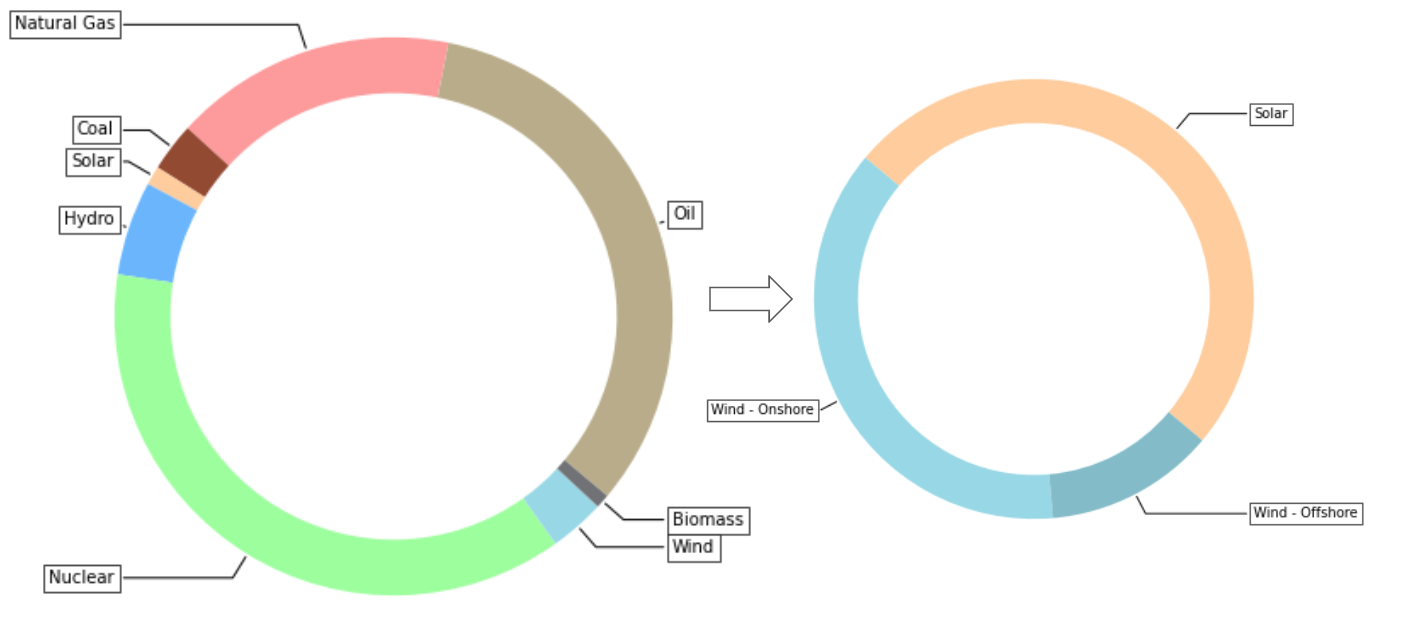
\includegraphics[width=\linewidth]{transition_s2a_smaller}
%$\big\Downarrow$
%    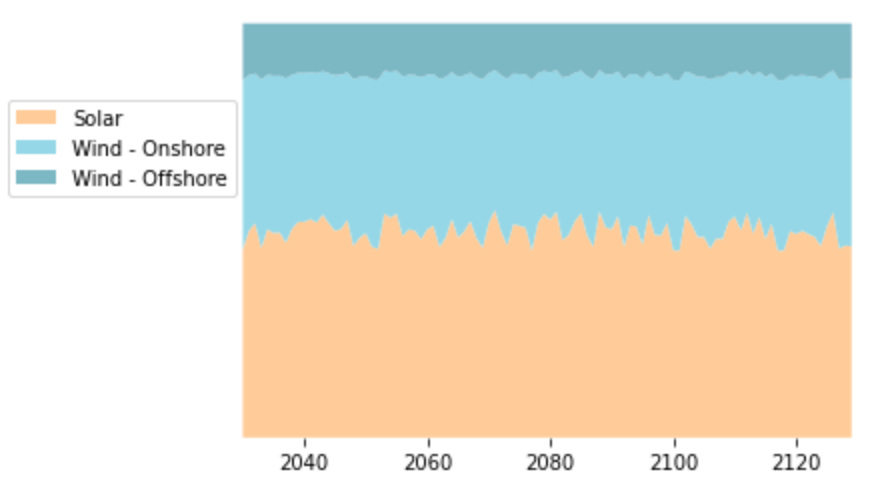
\includegraphics[width=\linewidth]{future_mix_s2a}
\end{center}
%\vspace{-2pt}
Note that in the French current energy mix above, Solar and Wind energies represent a small fraction of our current consumption. We can quickly see that the mere thought of transitioning our energy can be sobering when we look back at the historical transitions rate. A complete transition will always seem easier at its beginning, but sustained rate of change rarely happen over long periods of time.

We assume an energy consumption of 2,800 TWh (approximate current value in France), and decrease it down to 2,000 TWh to account for the better electrical efficiency of non-heat conversion systems.

}


\headerbox{3. Controllability implications}{name=mcs,column=0,below=model,span=1}{

As we have discussed, we can hope, in a very optimistic scenario, to only need to backup 10\% of our consumption needs for a week. In order to do this, we need to store energy. In the following, we will assume that short term (on the order of minutes to hours) and long term storage (seasonality effect) are both covered by Lithium-Ion (Li-Ion) Battery technology.

%Photo attribution: https://www.shutterstock.com/g/petrmalinak
\begin{center}
    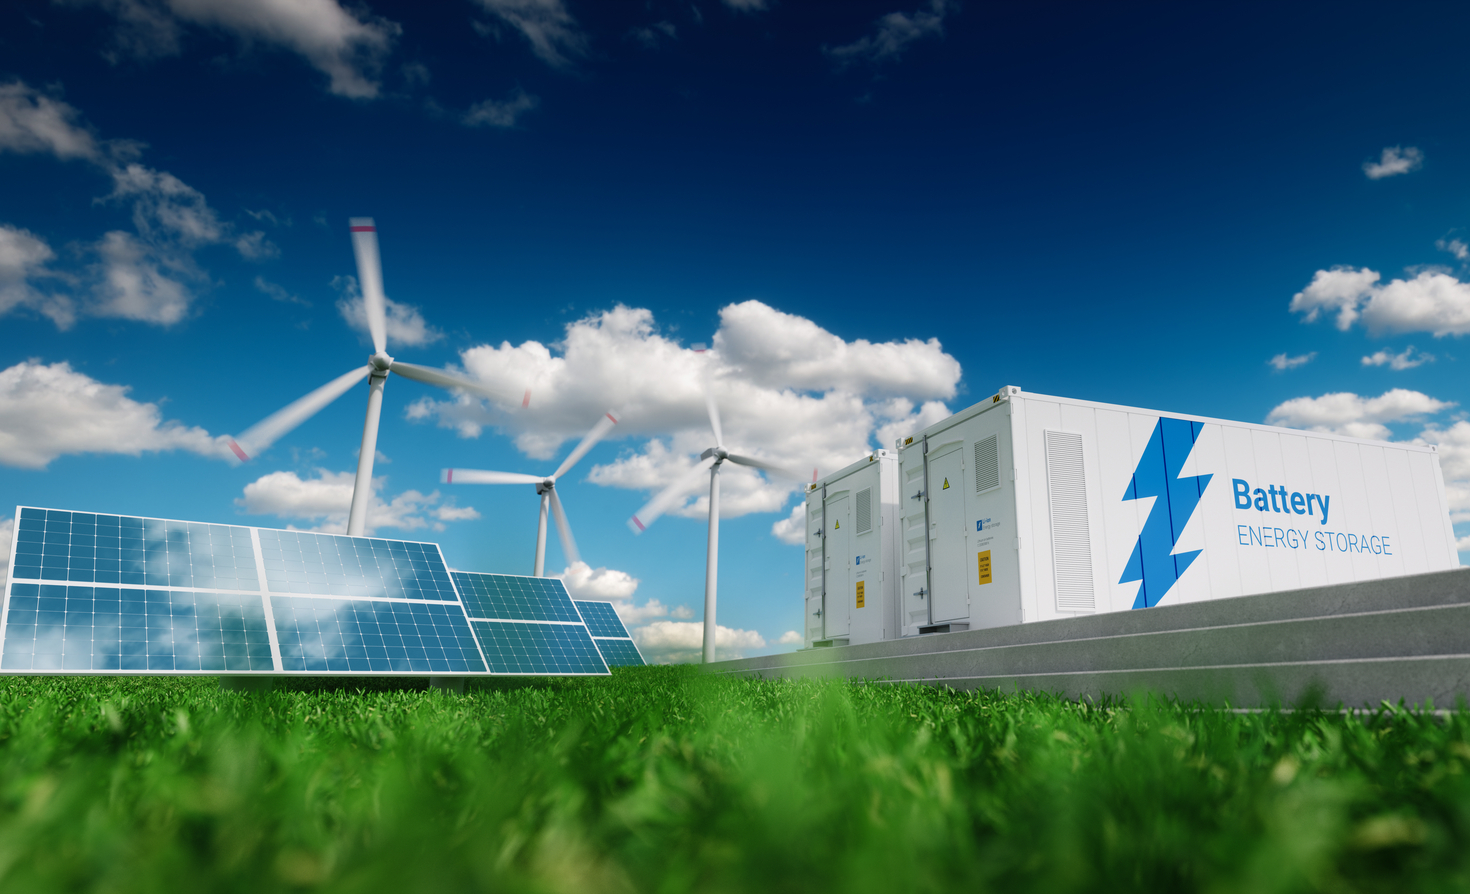
\includegraphics[width=\linewidth]{energystorageshutterstockpetrmalinak}
\end{center}
}

% Hydro image
%@article{bao2019debris,
%  title={Debris flow prediction and prevention in reservoir area based on finite volume type shallow-water model: a case study of pumped-storage hydroelectric power station site in Yi County, Hebei, China},
%  author={Bao, Yiding and Chen, Jianping and Sun, Xiaohui and Han, Xudong and Li, Yongchao and Zhang, Yiwei and Gu, Feifan and Wang, Jiaqi},
%  journal={Environmental Earth Sciences},
%  volume={78},
%  number={19},
%  pages={1--16},
%  year={2019},
%  publisher={Springer}
%}

% Battery image
%@article{goodenough2018we,
%  title={How we made the Li-ion rechargeable battery},
%  author={Goodenough, John B},
%  journal={Nature Electronics},
%  volume={1},
%  number={3},
%  pages={204--204},
%  year={2018},
%  publisher={Nature Publishing Group}
%}

\headerbox{4. Computations}{name=screen,span=2,column=1,below=introduction}{ % To reduce this block to 1 column width, remove 'span=2'

This scenario would imply the installation of around 350 GW of onshore wind,  75 GW of offshore wind, and 800 GW of solar. On top of this, one would need to account for energy storage, which translates to around 4 TWh. We use the current costs of solar system, wind farms, and battery systems to derive an economics approximation. The carbon emissions of this transition are also computed, as are some materials requirements.

\vspace{-5pt}
\begin{center}
    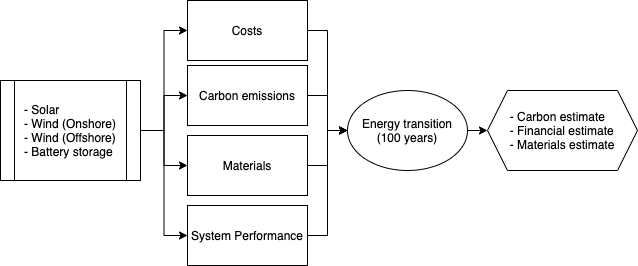
\includegraphics[width=0.85\linewidth]{algorithm_simple_scenarios}
\end{center}
}


\headerbox{5. Results and Limitations}{name=sea,span=2,column=1,below=screen}{ % To reduce this block to 1 column width, remove 'span=2'

The long term transition considered here to a 100\% renewable mix system would come at a cost of approximately \$16 trillions over the century. The carbon emissions would decrease to about 70 MT per year, as opposed to the current 300 MT per year. More problematic even than the price tag, France would need to use almost 10\% of the total world reserve of Dysprosium, and around 5\% of the total world resources of Lithium and Neodymium.

One thing to note is that the USA have an energy need approximately 10 times as large as France today. To transition them to our simplified scenario, take the previous calculation, and multiply basically everything by 10. This will give a good idea of the scale of the issue, notably in terms of materials resources. If France and the USA alone picked that simplified scenario, roughly all of the Dysprosium reserves would be gone well within the century, and more than half the hypothetical reserves of Lithium. This would represent the energetic transition of 5\% of the world population\ldots

\begin{kaobox}[frametitle=Common Questions]
\begin{itemize}
\item \textit{What about pumped storage to replace the batteries?}

Pumped storage is tackled in another Case Study. The short story is, the scale of the dams to build would make every other large project in history look pitiful.

\item \textit{What about Hydroelectricity and Biomass on top of Solar and Wind?}

Hydroelectricity and biomass would help reduce the need for batteries even more for the long term option, but the high variability of wind and solar does not make this solution solid, as you inherently need energy storage. \textbf{But, of course, the more varied (and clean) you are, the better}.

\item \textit{What about the other type of batteries, besides Li-Ion?}

The same materials limitations are encountered, notably Lead-Acid, the second most popular option.

\item \textit{What about hydrogen?}

Hydrogen production is a very interesting technology. It is today limited due to its reliance on Platinum for an efficient process, as well as its storage challenges. It is definitely worth pursuing, as are most clean technologies.

\end{itemize}
\end{kaobox}

}


\headerbox{6. Conclusions}{name=conclusion,column=1,below=sea,span=2,above=bottom}{
% DeCAF is a chemoinformatical tool that can be helpful in ligand-based drug design.
% It provides a comprehensive molecule description and a fast algorithms for comparing and aligning multiple ligands.
\begin{boenumerate}\compresslist
    \item The costs of a transition, while huge and important, are only one facet of the transition.
    \item Keep in mind that renewable energy does not mean renewable ways of capturing it
    \item You will hear more and more about the \textit{Finite Materials Problem}. This alone makes the specific scenario considered physically impossible, or rather implausible bar an unexpected breakthrough.
\end{boenumerate}
}


\headerbox{7. Go further}{name=references,column=0,span=1,below=mcs,above=bottom}{
Link to the Pumped Storage Case Study

Link to the Materials limitation Case Study

}

\end{poster}

\end{document}
